
\chapter{Segmentation}

Segmentation of medical images is a challenging task. A myriad of different
methods have been proposed and implemented in recent years. In spite of the
huge effort invested in this problem, there is no single approach that can
generally solve the problem of segmentation for the large variety of image
modalities existing today.

The most effective segmentation algorithms are obtained by carefully
customizing combinations of components. The parameters of these components are
tuned for the characteristics of the image modality used as input and the
features of the anatomical structure to be segmented.

The Insight Toolkit provides a basic set of algorithms that can be used to
develop and customize a full segmentation application. Some of the most
commonly used segmentation components are described in the following
sections.


\section{Region Growing}

Region growing algorithms have proven to be an effective approach for image
segmentation. The basic approach of a region growing algorithm is to start
from a seed region (typically one or more pixels) that are considered to be
inside the object to be segmented. The pixels neighboring this region are
evaluated to determine if they should also be considered part of the
object. If so, they are added to the region and the process continues as long
as new pixels are added to the region.  Region growing algorithms vary
depending on the criteria used to decide whether a pixel should be included
in the region or not, the type connectivity used to determine neighbors, and
the strategy used to visit neighboring pixels.

Several implementations of region growing are available in ITK.  This section
describes some of the most commonly used.

\subsection{Connected Threshold}

A simple criterion for including pixels in a growing region is to evaluate
intensity value inside a specific interval.

\label{sec:ConnectedThreshold}
\input{ConnectedThresholdImageFilter.tex}

\subsection{Otsu Segmentation}
Another criterion for classifying pixels is to minimize the error of misclassification.
The goal is to find a threshold that classifies the image into two clusters such that
we minimize the area under the histogram for one cluster that lies on the other cluster's
side of the threshold. This is equivalent to minimizing the within class variance
or equivalently maximizing the between class variance.

\label{sec:OtsuThreshold}
\input{OtsuThresholdImageFilter.tex}

\label{sec:OtsuMultipleThreshold}
\input{OtsuMultipleThresholdImageFilter.tex}

\subsection{Neighborhood Connected}
\label{sec:NeighborhoodConnectedImageFilter}
\input{NeighborhoodConnectedImageFilter.tex}


\subsection{Confidence Connected}
\label{sec:ConfidenceConnected}
\input{ConfidenceConnected.tex}
\subsubsection{Application of the Confidence Connected filter on the Brain Web Data}
This section shows some results obtained by applying the Confidence Connected filter on the BrainWeb database. The filter was applied on a 181 $\times$ 217 $\times$ 181 crosssection of the \textit{brainweb165a10f17} dataset. The data is a MR T1 acquisition, with an intensity non-uniformity of 20\% and a slice thickness 1mm. The dataset may be obtained from
\code{https://www.bic.mni.mcgill.ca/brainweb/} or
\code{https://data.kitware.com/\#folder/5882712d8d777f4f3f3072df}

The previous code was used in this example replacing the image dimension by 3.
Gradient Anistropic diffusion was applied to smooth the image. The filter used 2 iterations, a time step of 0.05 and a conductance value of 3. The smoothed volume was then segmented using the Confidence Connected approach. Five seed points were used at coordinate locations (118,85,92), (63,87,94), (63,157,90), (111,188,90), (111,50,88). The ConfidenceConnnected filter used the parameters, a neighborhood radius of 2, 5 iterations and an $f$ of 2.5 (the same as in the previous example). The results were then rendered using VolView.

Figure~\ref{fig:3DregionGrowingScreenshot1} shows the rendered volume. Figure~\ref{fig:SlicesBrainWeb} shows an axial, sagittal and a coronal slice of the volume.

\begin{figure}
\centering
\includegraphics[width=0.6\textwidth]{3DregionGrowingScreenshot1.eps}
\itkcaption[Whitematter Confidence Connected segmentation.]{White matter segmented using Confidence Connected region growing.}%
\label{fig:3DregionGrowingScreenshot1}
\end{figure}

\begin{figure}
\centering
\includegraphics[width=\textwidth]{SlicesBrainWebConfidenceConnected.eps}
\itkcaption[Axial, sagittal, and coronal slice of Confidence Connected segmentation.]{Axial, sagittal and coronal slice segmented using Confidence Connected region growing.}%
\label{fig:SlicesBrainWeb}
\end{figure}



\subsection{Isolated Connected}
\label{sec:IsolatedConnected}
\input{IsolatedConnectedImageFilter.tex}


\subsection{Confidence Connected in Vector Images}
\label{sec:VectorConfidenceConnected}
\input{VectorConfidenceConnected.tex}


\section{Segmentation Based on Watersheds}
\label{sec:WatershedSegmentation}
%
%
%  This file is inserted in the file Segmentation.tex
%
%

\subsection{Overview}
\label{sec:AboutWatersheds}
\index{Watersheds|textbf}
\index{Watersheds!Overview}

Combining differential expressions (such as the Laplacian) with linear or
nonlinear filtering in itself provides a variety of mechanisms for 2D and 3D
image segmentation.  This is done by combining edge detection with flood-fill
operations or by using inequalities to divide images into light and dark
regions (or positive and negative curvatures).  These methods can be effective
and are part of the Insight toolkit, but from our work with medical images we
have concluded that {\em watershed regions} (also called {\em catchment
basins}) are a powerful, flexible, and robust tool for image segmentation.
Watershed regions are formed by using the local geometric structure to
associate points in the image domain with local extrema in some feature
measurement.  This technique is less sensitive to user-defined thresholds, is
better suited for fusing different types of features from different data sets,
and naturally produces a hierarchy of segmentations from which a single
segmentation can be extracted either a-priori, using a threshold, or
interactively with the help of a graphical user interface \cite{Yoo1992,Yoo1991}.

The strategy of watershed segmentation is to treat an image $f$ as a height
function, i.e.  the surface formed by graphing $f$ as a function of its
independent parameters, $\vec{x} \in U$.  The image in question may not
necessarily be the original input data, but could be derived from that data,
through some filtering, graded (or fuzzy) feature extraction, or fusion of
feature maps from different sources.  The assertion is that higher values of
$f$ (or $-f$) indicate the presence of boundaries in the original data.

The strategy is to associate regions with local minima of $f$ (clearly interior
points) using the watersheds of the graph of $f$, as in
Figure~\ref{fig:segment}.
\begin{figure}
\centering
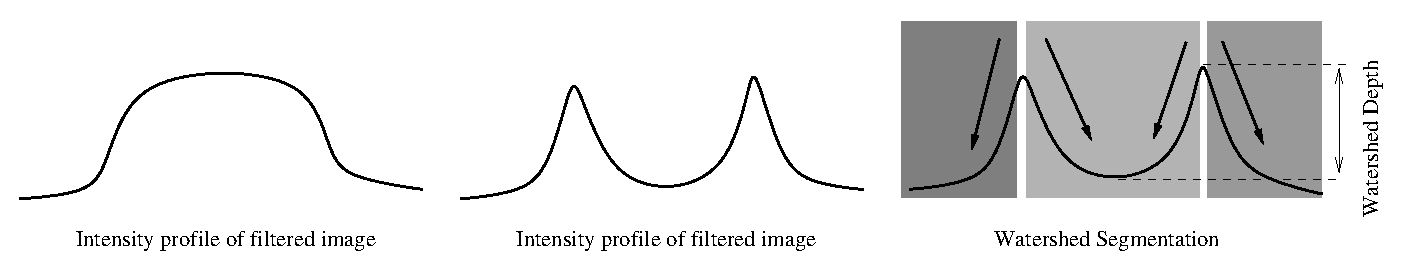
\includegraphics[width=0.9\textwidth]{WatershedCatchmentBasins.eps}
\caption{A fuzzy-valued boundary map, from an image or set of images, 
is segmented using local minima and catchment basins.}
\protect\label{fig:segment}
\end{figure}
That is, a segment consists of all points in $U$ whose paths of steepest
descent on the graph of $f$ terminate at the same minimum in $f$.  Thus, there
are as many segments in an image as there are minima in $f$.  The segment
boundaries are ``ridges'' \cite{Koenderink1979,Koenderink1993,Eberly1996} in
the graph of $f$.  In the 1D case ($U \subset \Re$) the watershed boundaries
are the local maxima of $f$, and the results of the watershed segmentation is
trivial.  For higher-dimensional image domains, the watershed boundaries are
not simply local phenomenon, they depend on the shape of the entire watershed.
In short, watershed segmentation has proven to be a sensible, reliable,
principled method for partitioning images that relies only on fuzzy-valued
boundary measurements.

The drawback of watershed segmentation is that it produces a region for each
local minimum, which is often, in practice, too many regions---an over
segmentation.  To alleviate this, we can establish a minimum watershed depth.
The watershed depth is the difference in height between the watershed minimum
and the lowest boundary point.  That is, the maximum depth of water a region
could hold without flowing into any of its neighbors.  Thus, a watershed
segmentation algorithm can sequentially combine watersheds whose depths fall
below the minimum until all of the watersheds are of sufficient depth.  This
depth measurement can be combined with other saliency measurements, such as
size.  The result is a segmentation containing regions whose boundaries and
size are significant.  Because the merging process is sequential, it produces a
hierarchy of regions, as shown in Figure~\ref{fig:watersheds}.
\begin{figure}
\centering
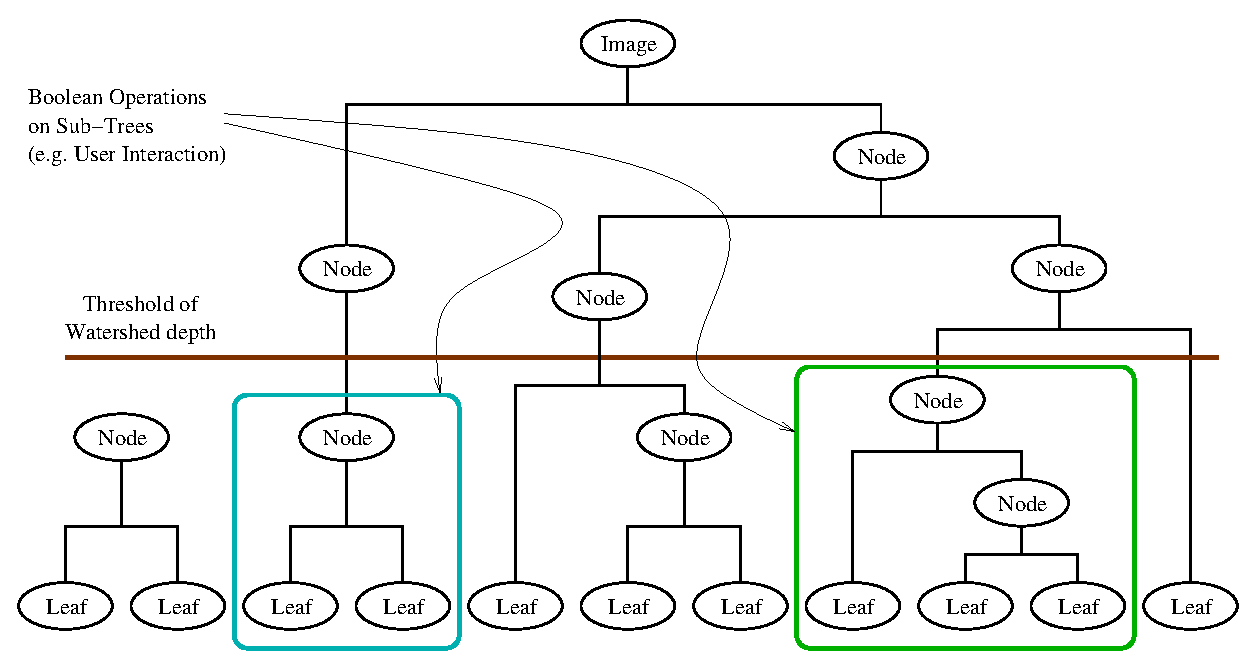
\includegraphics[width=0.9\textwidth]{WatershedsHierarchy.eps}
\caption{A watershed segmentation combined with a saliency measure 
(such as depth) produces a hierarchy of regions.  Structures can be 
derived from images by either thresholding the saliency measure or 
combining subtrees within the hierarchy}
\protect\label{fig:watersheds}
\end{figure}
Previous work has shown the benefit of a user-assisted approach, which provides
a graphical interface to this hierarchy so that a technician can quickly move
from the small regions that lie within a area of interest to the union of
regions that correspond to the anatomical structure \cite{Yoo1991}.

There are two different algorithms for implementing watersheds.  The bottom up
strategy starts with seeds at the local minima in the image and grows regions
outward and upward at discrete intensity levels (i.e., raises the water within
each watershed).  This approach, which limits the accuracy by enforcing a set
of discrete gray levels in the image, is equivalent to a sequence of
morphological operations (sometimes called {\em morphological watersheds}
\cite{Serra1982}).  Because we are considering the output of multi-scale
differential operators, the $f$ in question will have floating point values,
and therefore we use a top-down approach, which is to trace each point using a
steepest descent to a local minimum (or previously labeled region).  If done
properly, it requires visiting each of the pixels in the image domain only
once.  When implementing watershed segmentation in this fashion, care must be
taken in handling the boundaries of regions, in confronting perfectly flat
regions, and in determining the watershed depth, or order to produce consistent
results.

Figures~\ref{fig:WatershedColorSegmentation1}--~\ref{fig:WatershedColorSegmentation3}
\begin{figure}
\centering
\includegraphics[width=0.9\textwidth]{WatershedColorEdges.eps}
\caption{
A segmentation (white lines are segment boundaries) based on 
the gradient magnitude of a color image that has been processed with 
vector-valued anisotropic diffusion.}
\protect\label{fig:WatershedColorSegmentation1}
\end{figure}
\begin{figure}
\centering
\includegraphics[width=0.4\textwidth]{WatershedSpine1.eps}
\includegraphics[width=0.4\textwidth]{WatershedSpine1.eps}
\caption{
Insets from the segmentation of the color image shown in 
Figure~\protect\ref{fig:WatershedColorSegmentation1} at two different levels of 
watershed depth.  Top) A lower threshold partitions the spinal cord
into several distinct tracts.  Bottom) At a higher threshold the 
vertebrae becomes a single segment and the parts of the 
spinal cord merge.
}
\protect\label{fig:WatershedColorSegmentation2}
\end{figure}

\begin{figure}
\centering
\includegraphics[width=0.4\textwidth]{WatershedColorInput.eps}
\includegraphics[width=0.4\textwidth]{WatershedColorGradientMagnitude.eps}
\caption{
Inputs for the segmentation presented in \ref{fig:WatershedColorSegmentation3}.
Left) Cryogenic data set after smoothing with anisotropic diffusion.  Right)
Squared magnitude of gradients on every color channel.}
\protect\label{fig:WatershedColorInput}
\end{figure}


\begin{figure}
\centering
\includegraphics[width=0.4\textwidth]{WatershedArm1.eps}
\includegraphics[width=0.4\textwidth]{WatershedArm2.eps}
\caption{
Insets from the segmentation of the color image shown in 
Figure~\protect\ref{fig:WatershedColorSegmentation1} at two different levels of 
watershed depth.  Top) The fat around the arm consists of many 
distinct regions.  Bottom) At a higher threshold the 
fat becomes a single segment as do the bones.
}
\protect\label{fig:WatershedColorSegmentation3}
\end{figure}

show the results of segmenting the color image from
Figure~\ref{fig:WatershedColorInput}(a).  These results are obtained by
applying the watershed algorithm to the root-sum-of-squares gradient magnitude
shown in Figure~\ref{fig:WatershedColorInput}(b).  By changing the threshold on
the minimum watershed depth, we can obtain different degrees of segmentation.
No one segmentation is ``perfect''; at one level the spinal cord is segmented
into various tracts, while at another level it comes together to form a single
structure.  Smaller regions can be expanded into larger regions by either
changing the depth threshold or combining them under some user direction.

\subsection{Watershed Segmentation in Insight}
\label{sec:ImplementationWatersheds}
\index{Watersheds!Segmentation}
The Insight Toolkit implementation of the watersheds algorithm is based on the
top-down approach.  That is, it traces gradient descent down from image ridges
to local minima when identifying catchment basins (see the previous
section). The Insight implementation has been fully generalized to images of N
dimensions.  It is implemented as a standard image-to-image pipeline filter.
A scalar height image is passed into the filter and the filter produces a
labeled image at a user-specified minimum watershed depth as output.

The Insight algorithm was designed to be streamable.
What this means is that a dataset can be processed in discrete pieces and
joined back together again to produce the final result.  The streaming
algorithm is made possible by keeping track of gradient descent flows across
the piece-wise boundaries, then merging those segments which flow into one
another in a second pass through the data.  In practice, we have found that
streaming is only warranted when looking at very large datasets where available
computer memory may be a limiting factor (gigabyte portions of the Visible
Human color cryosection data, for example).  We have found, however, that for
very large datasets, the complexity of the algorithm makes it a less desirable
approach to segmentation.  For more information on the streaming possibilities
of the Insight watersheds algorithm, see the ``StreamedWatershedSegmentation''
example in the Insight code repository.

The watersheds algorithm uses a city-block connectivity when tracing gradient
descent flows.  This means that in 2D images the segmented regions are
4-connected, and in 3D images the segmented regions are 6-connected.  While
there is currently no API exposed to the user for changing connectivity, the
code was designed to be easily modified at the developer level to handle
arbitrary connectivities by replacing the connectivity object used in the
gradient descent stage of the algorithm.

There are several terms that it is worthwhile to clarify when discussing the
the watersheds algorithm.  In the context of the Insight
implementation, we refer to the input as the {\em height function}. The
watershed depth described in the previous section is sometimes called the
{\em flood level}, and is simply referred to as the {\em level} in the API of the
Insight watershed filter itself.  The collection of local minima and their
associated pixels (catchment basins) is called the {\em basic segmentation}.
The process of combining catchment basins in the basic segmentation to produce
larger segments according to minimum watershed depth and/or other saliency
measures is referred to as {\em merging}.  The hierarchy of merges that produce
segmentations at increasing flood level scales is called the {\em merge tree} or
the {\em merge hierarchy}.

\begin{figure}
\centering
\includegraphics[width=0.9\textwidth]{WatershedImageFilter.eps}
\caption{The construction of the Insight watersheds filter.}
\protect\label{fig:constructionWatersheds}
\end{figure}

Figure~\ref{fig:constructionWatersheds} shows how the Insight image-to-image
watersheds filter is constructed.  The filter is actually a collection of
smaller filters which perform the various steps of the watershed algorithm.  A
height image is fed to the input of the filter and the Segmenter object creates
the basic segmentation by tracing all pixels via steepest descent to their
local minima.  A low pass thresholding step precedes the gradient descent to
minimize the presence of shallow background regions, which result in
oversegmentation of the image and increased computation time.  The basic
segmentation is passed to a sub-filter which generates the merge tree up
to a user-specified maximum level.  The merge tree is then used by the image
relabeler to effect merging of segments in the basic segmentation and
produce an output image that is labeled at the desired scale.

Only three parameters control this filter.  They are shown in the
Figure~\ref{fig:constructionWatersheds} connected to the stages of processing
that they affect.  The relabeler is the main control point for GUI
interaction with the filter.  Once a merge tree has been generated, the {\em
output flood level} parameter can be raised and lowered anywhere below the {\em
maximum flood level} to generate a new labeled image in real-time.

\subsection{Using the Insight Watershed Filter}
\label{sec:UsingWatersheds}
\index{Watersheds!ImageFilter}
Because the Insight watershed filter has so few parameters\footnote{There is
really only one parameter, \emph{flood level}.  The \emph{threshold} parameter
is just another stage of preprocessing.}, the quality of a segmentation
correlates strongly with the quality of the height function that is given as
input. What quality means in this context is relative to the particular result
you are trying to achieve.

As noted in Section~\ref{sec:AboutWatersheds}, the input height function
should have strongly positive values at object boundaries.  A suitable height
function for many applications can be generated as the gradient magnitude of
the image.  The gradient magnitude image has the property that larger values
correspond to edges in the image.  Typically, the best results are obtained by
filtering the image first to remove high frequency components.  This is best
accomplished by using one of Insight's anisotropic diffusion filters, which
preserve edge features in the data while smoothing elsewhere.  The Insight
watershed filter expects real-valued, single component, scalar data as input.
The height image should be of floating point type.

Tuning the parameters is a process of trial and error.  The {\em threshold}
parameter can be used to great effect in controlling oversegmentation of the
image.  This reduces computation time and can produce a much cleaner output.
The trick is to get an understanding of the scale level of the objects in your
image.  The best time/quality trade-off is achieved when the image is smoothed
and thresholded to eliminate features which are just below the scale levels of
interest.

Fast resegmentation at different flood levels can be achieved by manipulating
the flood level parameter of the filter.  After generating a merge tree for a
segmentation at a given scale level, the filter can relabel the output at any
scale level contained in the merge tree in real-time (speed depends on the size
of the data set and the number of segments in the basic segmentation).  This
fast relabeling feature is useful for GUI-based applications and data
visualization.

Most of the computational complexity of the watersheds algorithm as it is
currently implemented in Insight comes from generating the merge hierarchy.
Processing times for this stage are exponential with respect to the number of
catchment basins in the basic segmentation. This means that increasing image
size does not necessarily slow processing times non-linearly.  Instead, the
execution speed decreases exponentially with information content in the image.
A very large, but very flat input may process in a much shorter time than a
very small, but very detailed input.  In practice, however, very large volumes
do tend to decrease merge times exponentially because scale of the segmented
objects does not usually change with image size.  When going from 2D to 3D (and
higher), increased interconnectivity of catchment basins in the basic
segmentation also leads to increases in processing time which are non-linear
with respect to the increased size of the data set.

\subsection{Visualizing the Results}
\label{sec:VisualizingWatersheds}
\index{Watersheds!Visualization}
In order to interpret the output of the Insight watersheds algorithm, it is
important to understand what the output is and how it is encoded.  The
watersheds image filter produces an image of unsigned long integers.  This
output is the same size and dimensionality of the input image.  Each integer
number is a label for a different segmented region (catchment basin) of the
original input.  

Because the segmented image may have potentially many thousands of discrete
unsigned long values, some care must be taken when visualizing the
data. Conversion to an image format with 255 gray levels is not recommended
because much of the information content of the segmentation could be lost.  One
effective way to visualize the output is to map the integer labels into
distinct RGB colors.  Because labels close in value tend to also be close
spatially in the image, it is helpful to spread close values far apart in
the RGB range.  A hashing scheme that puts more weight on the least-significant
integer bits is a good way to accomplish this.  Figure~\ref{fig:colorVisWatersheds} 
shows a slice taken from a segmentation of a section of abdomen from the Visible Female
Cryosection data.  The unsigned long label values of the output have been
hashed into RGB colors.

\begin{figure}
\centering
\includegraphics[width=.95\textwidth]{WatershedAbdomenSegmentation.eps}
\caption{A slice from a segmentation of Visible Female cryosection data.
The original is shown at the left and the segmented image is shown to the
right. Colored regions in the segmented image correspond to structures in the
original data. }
\protect\label{fig:colorVisWatersheds}
\end{figure}

For volumetric data, it is often interesting to create a surface rendering of
one or more regions in the output.  This can be done by thresholding the
region(s) of interest from the output image and exporting the result to a
visualization package capable of isosurface rendering.  Thresholding can be
done either by explicit manipulation of the image values\footnote{Using the
\code{itk::ImageRegionIterator}, visit each image pixel and assign all values not
equal to the labels of interest to 0.} or through one of the several Insight
image thresholding filters.  The thresholded data can be written to a file and
read in to other image processing or visualization packages.  There is also
support for exporting Insight data to other packages at run-time (see the
itk::ExportImageFilter for more information).
Figure~\ref{fig:surfaceRenderingWatersheds} is a surface rendering of the right
eye, the optic nerve and chiasm, the lens of the eye, and the right lateral
rectus muscle.  A slice from the original Visible Female head and neck
cryosection data from which the segmentations were created is shown at the
left.  This image was created as described above by thresholding isovalues in a
watershed segmentation output and rendered using the Visualization Toolkit
(VTK).  Before rendering, the volume was antialiasing with
\code{itk::AntialiasBinaryImageFilter}.


\begin{figure}
\centering
\includegraphics[width=0.95\textwidth]{WatershedRendering.eps}
\caption{A surface rendering (right) of four anatomical structures in the Visible
Female head and neck. A slice of the data from which the segmentation was
created is shown at the left.  The right and left optic nerves and chiasm are
shown in yellow.  The right eye is in transparent purple.  The lens is dark
purple.  The structure in red is the lateral rectus muscle.}
\protect\label{fig:surfaceRenderingWatersheds}
\end{figure}

The watershed algorithm is automatic in that it does not require the user to
input seed points or specify many parameters, but we have found that the best
segmentations are obtained when the algorithm can be used interactively.  Given
a graphical interface to the merge hierarchy, a technician can quickly
resegment the data at different watershed depth levels and choose the regions
that best represent structures of interest in the data.  The Insight
repository contains an example segmentation application that allows real-time
manipulation of watersheds output to construct binary volume segmentations.
This application is covered in more detail in the next section.

\subsection{Interactive Segmentation}
\label{sec:SegmentationEditorWatersheds}
\index{Watersheds!Segmentation Editor}
The Segmentation Editor (SE) example in the Insight repository is a complete
system for interactively segmenting image data using the watersheds algorithm.
The goal of the software is to combine human interaction with automated image
processing techniques to produce a better result than either technique can give
on its own. The SE tool is a test of the hypothesis that through image analysis
and targeted visualization of the data, the task of hand labeling voxels
contained in anatomical structures can be more efficient than hand segmentation
alone.  The application also serves as a testbed for development of new
segmentation techniques and algorithms.

The SE application was originally created for use in algorithm validation
studies.  Validation studies are an important part of the Insight project.
Algorithms that we have developed are tested on real clinical data and applied
to simulated clinical scenarios.  For the watersheds algorithm, we have applied
our interactive segmentation to problems of MRI tumor segmentation and the
creation of anatomical atlases from the Visible Female color cryosection data.
Complete reports on all of the validation studies for the initial phase of
Insight algorithm development are available as of the October 2002 release of
the toolkit.

The SE application is build in the Tcl scripting language.  The graphical
interface was constructed using a Tk.  Visualization is done with the
Visualization Toolkit (VTK) wrapped as Tcl commands.  The Insight filters used
in the application were wrapped first as VTK filters and then also as Tcl
commands.  Figure~\ref{fig:SegmentationEditorBuildWatersheds} shows how the
various components of the application are put together.

\begin{figure}
\centering
\includegraphics[width=0.90\textwidth]{WatershedSegmentationEditorBuild.eps}
\caption{A user interacts with the Segmentation Editor application.  User
commands cause updates in the Insight (ITK) and VTK pipelines, which are
connected through data export and import filters.}
\protect\label{fig:SegmentationEditorBuildWatersheds}
\end{figure}

Preprocessing image data correctly is important for achieving good segmentation
results with the watershed algorithm.  The SE application has a preprocessing
stage which filters using anisotropic diffusion and generates a height input
based on gradient magnitude.  As described in the preceding sections, this is a
good general purpose way to prepare image data for segmentations based on watersheds.
Figure~\ref{fig:preprocessWatersheds} shows the preprocessing stage of the
segmentation process.  The data shown is MRI data from the Harvard
Brigham and Women's Brain Tumor Database \cite{Kaus2001,Warfield2000b}.  At
left is a slice from the original data.  The center image has been diffused
with the Insight gradient-based anisotropic diffusion filter for 12 iterations
at a conductance coefficient of 1.0.  The rightmost image is the gradient
magnitude of the smoothed image.

\begin{figure}
\centering
\includegraphics[width=0.80\textwidth]{WatershedsPreprocessing.eps}
\caption{Preparing a height function for input to the watersheds algorithm.
The image on the left is a slice of the original MRI.  The image in the middle
is a slice of the data after 12 iterations of a gradient based anisotropic
diffusion filter (conductance term 1.0).  The right-most image is the gradient
magnitude of the diffused data.}
\protect\label{fig:preprocessWatersheds}
\end{figure}



The Segmentation Editor gets its name from the process of interacting with the
watersheds output to literally piece together a 3D segmentation.  Once the
watersheds algorithm has been run on the preprocessed data, the entire merge
hierarchy is made available to the user.  A segmentation is constructed by
selecting catchment basins from anywhere in the hierarchy and then adding them
to the segmentation.  Figure~\ref{fig:editingWatersheds} is a snapshot of the
SE tool.  The data shown in Figure~\ref{fig:preprocessWatersheds} has been
segmented.  At left is the segmentation output shown at the scale selected on
the ``scale'' slider of the console.  The colored regions represent catchment
basins available for selection.  In the center window, a selected region which
correspond to the location of the tumor has been overlain in blue on the
original data.  Only one slice of the data is displayed at a time, but the
3D surface of the tumor segmentation is rendered for reference.

\begin{figure}
\centering
\includegraphics[width=0.80\textwidth]{WatershedSegmentationApplicationGUI.eps}
\caption{Snapshot of the Segmentation Editor Tool}
\protect\label{fig:editingWatersheds}
\end{figure}




% the clearpage command helps to avoid orphans in the title of the next
% section.
\clearpage

\section{Level Set Segmentation}
\label{sec:LevelSetsSegmentation}
%%%%%%%%%%%%%%%%%%%%%%%%%%%%%%%%%%%%%%%%%%%%%%%%%%%%%%%%%%%%%%%%%%%%%%%%
%
%
%     This file is included from the file   Segmentation.tex
% 
%     Section tag and label are placed in this top file.
%
%
%
%%%%%%%%%%%%%%%%%%%%%%%%%%%%%%%%%%%%%%%%%%%%%%%%%%%%%%%%%%%%%%%%%%%%%%%%



\subsection{Threshold Level Set Segmentation}

\subsection{Fast Marching Segmentation}

\subsection{Shape Detection Segmentation}

\subsection{Geodesic Contours Segmentation}



\subsection{Segmentation Level Set Image Filter}
\label{sec:SegmentationLevelSetImageFilter}





%HACK: TODO Review what happened to these.
%REMOVED PATENTED: \section{Hybrid Methods}
%REMOVED PATENTED: \label{sec:HybridSegmentationMethods}
%REMOVED PATENTED:
%REMOVED PATENTED: %%%%%%%%%%%%%%%%%%%%%%%%%%%%%%%%%%%%%%%%%%%%%%%%%%%%%%%%%%%%%%%%%%%%%%%%
%
%
%     This file is included from the file   Segmentation.tex
% 
%     Section tag and label are placed in this top file.
%
%
%
%%%%%%%%%%%%%%%%%%%%%%%%%%%%%%%%%%%%%%%%%%%%%%%%%%%%%%%%%%%%%%%%%%%%%%%%

\subsection{Introduction}
\label{sec:HybridSegmentationIntroduction}


It is sometimes convenient to combine several segmentation strategies with the
aim of taking advantage of their qualities an compensate their vulnerabilities.
The synergy between fundamentally different methodologies tends to result in
robustness and higher segmentation quality.  This section illustrates an hybrid
approach for segmentation in which two different strategies are configured to
work together. In this case, an input image is first processed by a filter
based on the concept of region growing. The criterion of acceptance in the
region is defined by a similarity measure that evaluates how homogeneous is the
path between to pixels. The output of this filter is used as a prior for
another filter that performs a full partition of the image space and then work
joining and splitting regions in order to optimize an homogeneity measure.
Details on the concepts behind those methods have been discussed in the
litterature
\cite{Angelini2002,Udupa2002,Jin2002,Imielinska2001,Imielinska2000a,Imielinska2000b}



\subsection{Background}
\label{sec:HybridSegmentationBackground}




%%%%%%%%%%%%%%%%%%%%%%%%%%%%%%%%%%%%%%%%%%%%%%%%%%%%%%%%%%%%%%%%%
%
%  Here is an example of how to include diagram in a figure
%
%  The file HybridSegmentationDiagram1.fig should be in the "Art"
%  directory. CMake will convert it to EPS before running latex. 
%
%%%%%%%%%%%%%%%%%%%%%%%%%%%%%%%%%%%%%%%%%%%%%%%%%%%%%%%%%%%%%%%%%

\begin{figure}
\center
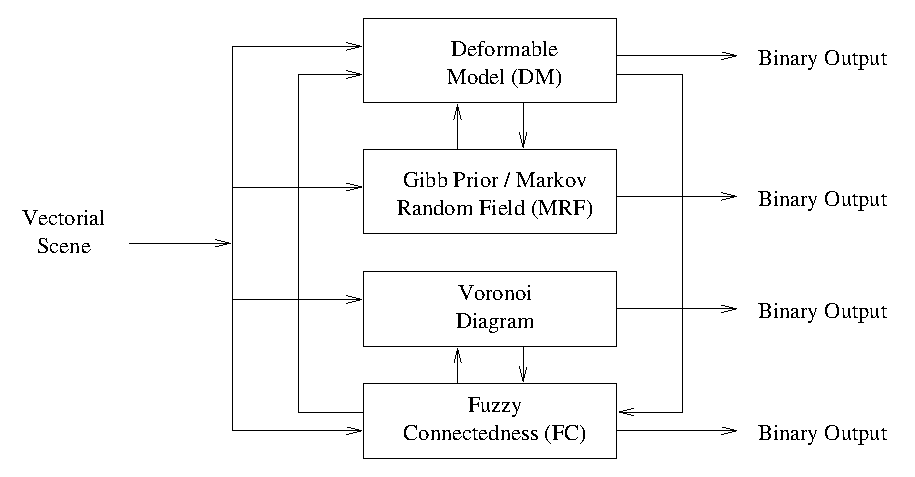
\includegraphics[width=6cm]{HybridSegmentationEngine1.eps}
\caption{Components of a HybridSegmentation approach}
\label{fig:HybridSegmentationEngine1}
\end{figure}

The Figure \ref{fig:HybridSegmentationEngine1} illustrates the main
components of the hybrid segmentation algorithm.

\begin{figure}
\center
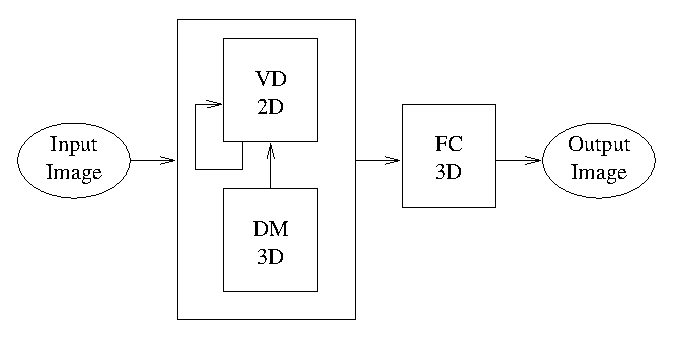
\includegraphics[width=6cm]{HybridSegmentationFCVDDM.eps}
\caption{Components of a HybridSegmentation approach}
\label{fig:HybridSegmentationFCVDDM}
\end{figure}


\begin{figure}
\center
\includegraphics[width=6cm]{VoronoiSegmentationClassDiagram1.eps}
\caption{UML Class Diagram of the VoronoiSegmentation filter}
\label{fig:VoronoiSegmentationClassDiagram1}
\end{figure}


\begin{figure}
\center
\includegraphics[width=6cm]{FuzzyConnectednessClassDiagram1.eps}
\caption{UML Class Diagram of the FuzzyConnectedness filter}
\label{fig:FuzzyConnectednessClassDiagram1}
\end{figure}


\begin{figure}
\center
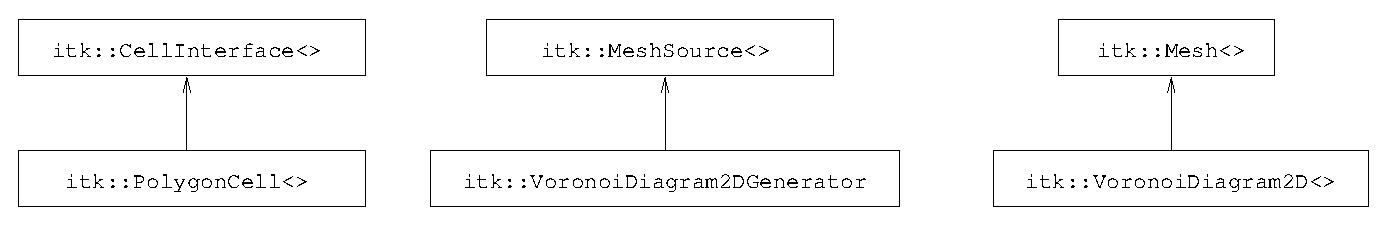
\includegraphics[width=6cm]{VoronoiSegmentationCollaborationDiagram1.eps}
\caption{UML Collaboration Diagram of the VoronoiSegmentation filter}
\label{fig:VoronoiSegmentationCollaborationDiagram1}
\end{figure}



\begin{figure}
\center
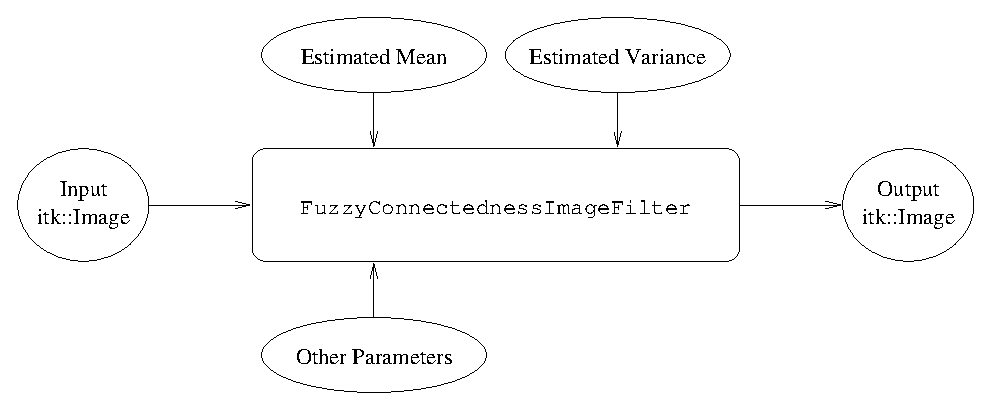
\includegraphics[width=6cm]{FuzzyConnectednessCollaborationDiagram1.eps}
\caption{UML Collaboration Diagram of the FuzzyConnectedness filter}
\label{fig:FuzzyConnectednessCollaborationDiagram1}
\end{figure}



\begin{figure}
\center
\includegraphics[width=6cm]{VoronoiSegmentationCollaborationDiagram2.eps}
\caption{UML Collaboration Diagram of the VoronoiSegmentation filter}
\label{fig:VoronoiSegmentationCollaborationDiagram2}
\end{figure}




\begin{figure}
\center
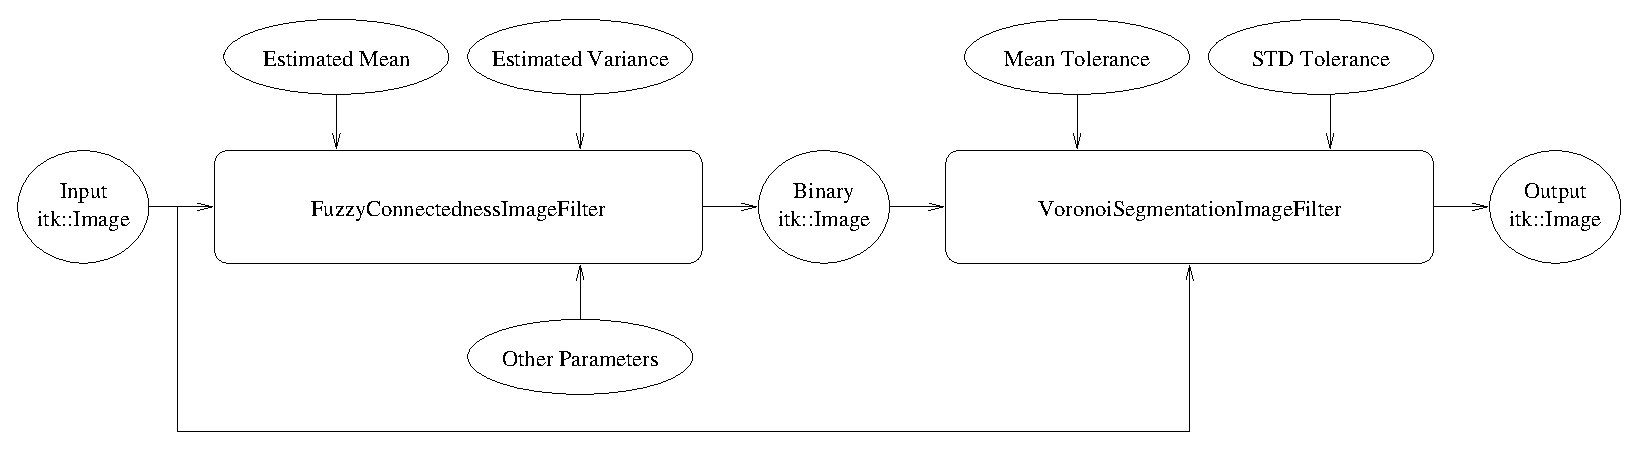
\includegraphics[width=6cm]{FuzzyVoronoiCollaborationDiagram1.eps}
\caption{UML Collaboration Diagram of the Fuzzy Voronoi Segmentation}
\label{fig:FuzzyVoronoiCollaborationDiagram1}
\end{figure}




\begin{figure}
\center
\includegraphics[width=6cm]{FuzzyVoronoiDeformableCollaborationDiagram1.eps}
\caption{UML Collaboration Diagram of the Fuzzy Voronoi Deformable Segmentation}
\label{fig:FuzzyVoronoiDeformableCollaborationDiagram1}
\end{figure}









%%%%%%%%%%%%%%%%%%%%%%%%%%%%%%%%%%%%%%%%%%%%%%%%%%%%%%%%%%%%%%%%%
%
%  Here is an example of how to include equations
%
%%%%%%%%%%%%%%%%%%%%%%%%%%%%%%%%%%%%%%%%%%%%%%%%%%%%%%%%%%%%%%%%%


\begin{equation}
MS(A,B) = \frac{1}{N} \sum_i^N \left( A_i - B_i \right)^2
\end{equation}





\subsection{Example}
\label{sec:HybridSegmentationExample1}

\input{HybridSegmentationFuzzyVoronoi.tex}





\section{Feature Extraction}
\label{sec:FeatureExtractionMethods}
%%%%%%%%%%%%%%%%%%%%%%%%%%%%%%%%%%%%%%%%%%%%%%%%%%%%%%%%%%%%%%%%%%%%%%%%
%
%
%     This file is included from the file   Segmentation.tex
%
%     Section tag and label are placed in this top file.
%
%
%
%%%%%%%%%%%%%%%%%%%%%%%%%%%%%%%%%%%%%%%%%%%%%%%%%%%%%%%%%%%%%%%%%%%%%%%%


Extracting salient features from images is an important task on image
processing.  It is typically used for guiding segmentation methods, preparing
data for registration methods, or as a mechanism for recognizing anatomical
structures in images. The following section introduce some of the feature
extraction methods available in ITK.


\subsection{Hough Transform}
\label{sec:HoughtTransform}

The Hough transform is a widely used technique for detection of geometrical
features in images. It is based on mapping the image into a parametric space
in which it may be easier to identify if particular geometrical features are
present in the image. The transformation is specific for each desired
geometrical shape.

\subsubsection{Line Extraction}
\label{sec:HoughtLineExtraction}
\input{HoughTransform2DLinesImageFilter.tex}


\subsubsection{Circle Extraction}
\label{sec:HoughtCircleExtraction}
\input{HoughTransform2DCirclesImageFilter.tex}

